\documentclass[t]{beamer}

% Indicate theme, etc.
\usetheme{default}
\setbeamerfont{frametitle}{size = \normalsize}
\setbeamerfont{caption}{size = \tiny}

% Import packages
\usepackage[utf8]{inputenc}
\usepackage{amsmath}
\usepackage{graphicx}
\usepackage{amssymb}
\usepackage{mathtools}
\usepackage[skip = 5pt]{caption}

% Define new commands
\newcommand{\norm}[1]{\lVert #1 \rVert}

% Begin document
\begin{document}

% Title slide
\title{Problem A - Conflict Between Patrilineal Clans}
\subtitle{2018 SCUDEM Competition}
\author{Sam Rosen \and Sharath Ramkumar \and Ji Hun Hwang}
\institute{University of Massachusetts: Amherst}
\date{October 2018}

\begin{frame}
\titlepage

\end{frame}

% Slide about Problem
\begin{frame}
\frametitle{Problem A: Conflict Between Patrilineal Clans}
\\
&
\\
There is evidence to suggest that the genetic variation in the Y chromosome decreased significantly 7,000 years ago because a large percentage of males died out due to conflict from warring patrilineal clans. \\~\\
We model a scenario of multiple clans of different sizes warring over territory.
\\
&
\\
We track the ratio of males to females for all groups to see how the distribution of the Y chromosome changes throughout time.

\vspace{2cm}
\begin{center}
\begin{figure}
\vspace{-2.1cm}
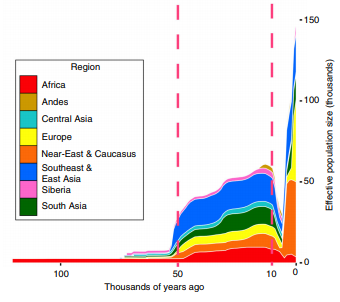
\includegraphics[scale=0.4]{malepop.png} % illustration of clans and location
\end{figure}
\end{center}

\end{frame}

% Slide 1
\begin{frame}
\frametitle{Initial Conditions and Assumptions}

\begin{itemize}
\item We are observing a square plot of land on Earth that contains each clan. The Earth is an infinite plane for simulation purposes.
\\
\item We have a given number of clans $n$; there will be no migration of clans.
\\
\item Each clan starts with some distinct initial population.
\\
\item Resources are evenly distributed among land and all land is equally viable for food. Each square unit of land supports a given number of people, $c$.
\\
\item Each clan starts at an initial location $(x,y)$ in the square and does not move.
\end{itemize}

\end{frame}

\begin{frame}{Initial Conditions and Assumptions - continued}
\begin{figure}
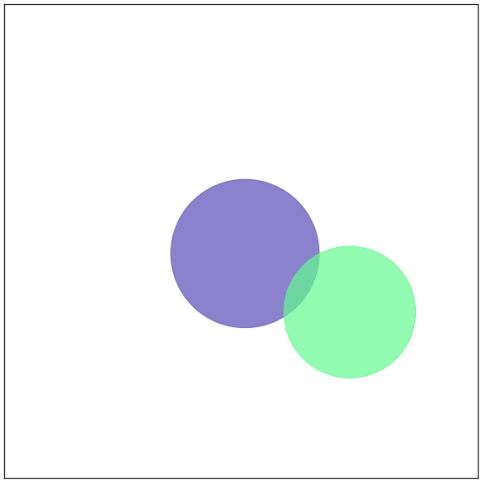
\includegraphics[scale=0.4]{diagram.png} % illustration of clans and location
\caption{Example of the world with two clans}
\end{figure}
\end{frame}

% Slide 2
\begin{frame}
\frametitle{Model Definition: Gender}
To model the change in gender for every clan it is useful to define the change in population for each clan as:

$$ \frac{dP_i}{dt} = \frac{dM_i}{dt} + \frac{dF_i}{dt} $$

and the percent female as 
$$s_i(t) = \frac{F_i(t)}{F_i(t) + M_i(t)} \in \left[0,1\right]$$
Where $M$ and $F$ represent the number of males and females respectively.

\end{frame}

% Slide 4
\begin{frame}
\frametitle{Model Definition: Logistic Growth and Gender}

The typical logistic function used to model population is:

$$\dfrac{dP}{dt} = rP\left(1 - \dfrac{P}{K}\right)$$

We define our carrying capacity as $K_{net} = c\;d^2$ where $c$ is the number of people supported by one square unit and $d$ is the side length of the square plot.

$$ r(s_i) = -s_i^3 \ln{(s_i)} $$
% \begin{tabular}{p{3cm}c}
% \begin{equation}
% r(s_i) = s_i^3 \ln{(s_i)}
% \end{equation}
% %&
% %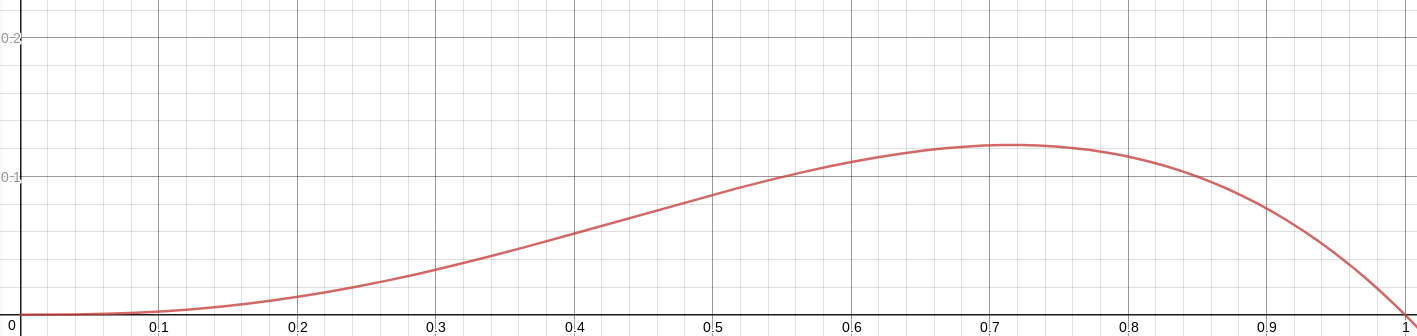
\includegraphics[scale=0.10]{r.png}
% \end{tabular}


We can finalize the growth part of the model for both males and females as below since all births will be split between the genders:

$$ \frac{dM_i}{dt}^{+} = \frac{dF_i}{dt}^{+} = \frac{1}{2}r(s_i)P_i\left(1 - \frac{P_i}{K_{net}}\right)$$


\end{frame}

% Slide 6
\begin{frame}
\frametitle{Model Definition: Clan Conflict}
To measure a clan's internal discontent we can measure its distance from carrying capacity.

$$\Delta_i = K_{net} - P_i(t)$$

When two clans have sufficient contact they may have conflict based on their discontent:

$$A_{i, j} = \left(\lambda_{i, j}\frac{1}{\ln(\Delta_i\Delta_j)}\right)^p$$

$\lambda_{i, j}$ can have multiple definitions as the measure of contact. We define it as the overlapping area between two clan's territories, calculated with the radii and centers.

$$P_i = c(Area) = c \pi r_i^2 \; \Rightarrow \; r_i = \sqrt{\dfrac{P_i}{c\pi}}$$

\end{frame}


% Slide 7
\begin{frame}
\frametitle{ODE's and Parameter Outline}

By summing up the conflict we now have a quantity for the decrease in rate or change for males and females.
\begin{align*}
    \frac{dM_i}{dt}
    &= \begin{cases}
        \dfrac{1}{2}r(s_i)P_i\left(1 - \dfrac{P_i}{K_{net}}\right) - g\displaystyle\sum\limits_{j \neq i} A_{i,j}, & F_i > 0 \\
        \eta M_i, & F_i \leq 0 % \\https://www.overleaf.com/project/5bce74f725621d76a6ce0458
    \end{cases}\\
    \frac{dF_i}{dt}
    & = \begin{cases}
        \dfrac{1}{2}r(s_i)P_i\left(1 - \dfrac{P_i}{K_{net}}\right) - \left(1-g\right)\displaystyle\sum\limits_{j \neq i} A_{i,j}, & M_i > 0 \\
        \eta F_i, & M_i \leq 0 \\
    \end{cases}
\end{align*}
% $$ \frac{dM_i}{dt} = \frac{dM_i}{dt}^{+} + \frac{dM_i}{dt}^{-} = \frac{1}{2}r(s_i)P_i\left(1 - \frac{P_i}{K_{net}}\right) - g\sum_{j \neq i} A_{i,j} $$

% $$ \frac{dF_i}{dt} = \frac{dF_i}{dt}^{+} + \frac{dF_i}{dt}^{-} = \frac{1}{2}r(s_i)P_i\left(1 - \frac{P_i}{K_{net}}\right) - (1-g) \sum_{j \neq i} A_{i,j} $$

\begin{itemize}
\item $g$ the percent of deaths through conflict that are male
\\
\item $\eta \in [-1,0]$ is a decaying factor for when births are no longer possible.
\end{itemize}

\end{frame}


\begin{frame}
{ODE's and Parameter Outline - Continued}

\begin{itemize}
\item $g = .85$ the percent of deaths through conflict that are male
\\
\item $\eta \in [-1,0], \eta = .7$ is a decaying factor for when the population growth is no longer possible.
\item $c = 5$ the number of people supported by one square unit of land
\\
\item $d = 100$ the side length of the square plot
\\
\item $p = 3$ the global hostility level
\\
\item Each clan has a Cartesian coordinate $(x,y)$, initial population, and initial gender ratio.
\end{itemize}

\end{frame}
% \begin{frame}{Simulation}
% Euler method (with $dt = 0.01$) implemented with Python3 was used to approximate the solution, and the initial conditions were chosen pseudo-randomly. 

% Each time step represents 10 years to approximate until $t = 700$, i.e. $700 \times 10 = 7000$ years.
% \begin{table}[!h]
%     %\centering
%     \begin{tabular}{|c|c|c|c|}\hline
%         Parameter & Symbol & Value/Range & Selected (if Global)\\ \hline
%         Dimension & $d$ & $100$ & $100$ \\ \hline
%         Density & $c$ & $\left(0, 10\right)$ & $7$ \\ \hline
%         Death Disparity & $g$ & $\left(0.5, 0.9\right)$ & $0.58$ \\ \hline
%         Hostility & $p$ & $\left(0, 10\right)$ & $3.4$ \\ \hline
%         Natural Death & $\eta$ & $\left(0, 1\right)$ & $0.7$ \\ \hline
%         Clan Center & $\left(x_i, y_i\right)$ & $\left(0, d\right)$ & - \\ \hline
%         Initial Population & $P_0$ & $\left(50, 100\right)$ & - \\ \hline
%     \end{tabular}
%     \caption{Parameters for Simulations}
%     \label{tab:parameters}
% \end{table}
% \end{frame}

% \begin{frame}{Simulation Results}

% \begin{itemize}
%     \item The clan that outnumbers (or has more males) another clan is most likely to be the winner of the conflict and reach the carrying capacity or stability. 
%     \item Since males have higher rate of death during the conflict, clans will reach $s_i = 1.0$ or very close before its elimination unless every member in the clan dies simultaneously. 
%     \item Winning clan reaches the equilibrium gender ratio once rest of the clan disappears. Equilibrium gender ratio is mostly found in the interval $s_{i_\text{eq}} \in [0.5,0.6]$.
% \end{itemize}

% \end{frame}


% Slide 7
\begin{frame}
\frametitle{Results: Two Clans}
Only one of the two clans are expected to survive unless two class has exactly same number of population and sex ratio, in which case two clans could oscillate and reach equilibrium. 

\begin{figure}
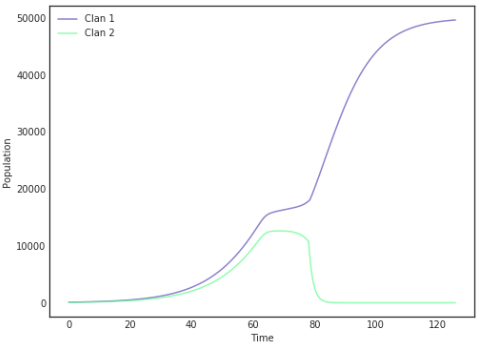
\includegraphics[width=5.2cm]{twoclanpop.png}
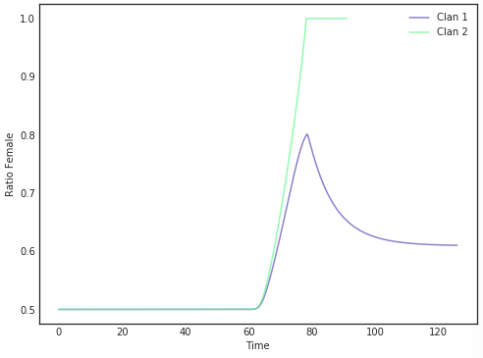
\includegraphics[width=5.2cm]{twoclanratio.png}
\caption{Population and gender ratio of clans by time when $n=2$.}
\end{figure}

\end{frame}

% Slide 7
\begin{frame}
\frametitle{Results: Multiple Clans ($n=8$)}
As before, eventually only one clan takes over everyone and reaches the carrying capacity, i.e. stability.

\begin{figure}
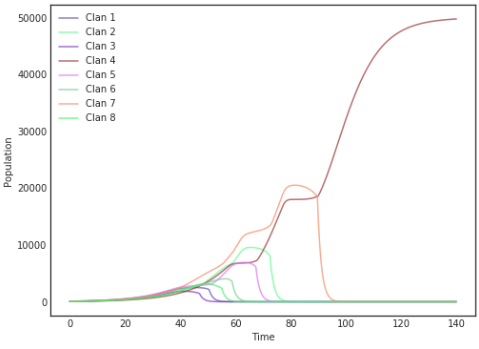
\includegraphics[width=5.2cm]{multclanpop.png}
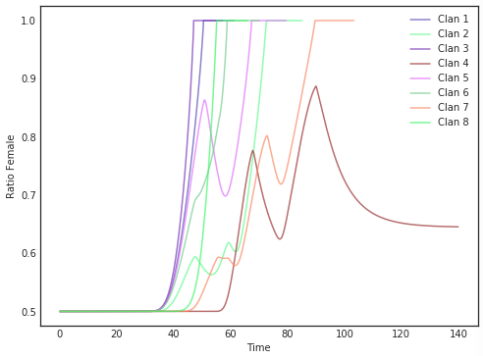
\includegraphics[width=5.2cm]{mclanratio.png}
\caption{Population and gender ratio of clans by time when $n=8$.}
\end{figure}

\end{frame}


% Slide 8
\begin{frame}
\frametitle{Supplemental Issue}
\textbf{What is the role of human mobility in the model?}\\~\\

We assume that larger groups travel slower than smaller groups and clans are moving in $x$ and $y$ directions independently. Our earlier model assumed stationary clans but the ability to add movement is possible by defining:

$$ \frac{dx_i}{dt} = \frac{dy_i}{dt} = \frac{\sqrt{\Delta_i}}{d}B = \frac{\sqrt{K_{net} - P_i}}{d}B$$
$$ B \sim Discrete Uniform[-1, 1]$$

\begin{itemize}
    \item As a group reaches carrying capacity, movement goes to zero. 
    \item Movement is scaled based on the size of the environment. 
    \item B is used to determine direction.
\end{itemize}

\end{frame}

% Slide 9
\begin{frame}
\frametitle{Supplemental Issue (Results)}

\begin{figure}
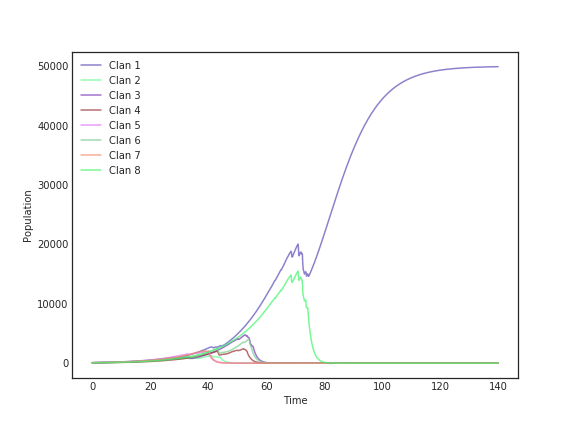
\includegraphics[width=5.2cm]{population_moving.png}
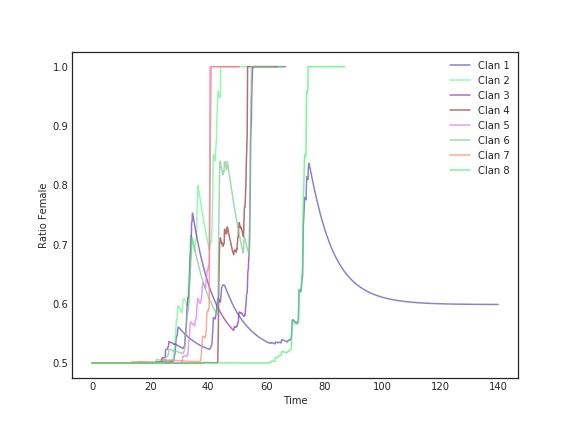
\includegraphics[width=5.2cm]{ratio_female_moving.png}
\caption{Population and gender ratio of clans by time when $n=8$ movement is accounted for.}
\end{figure}

\end{frame}


% Slide 10
\begin{frame}
\frametitle{Conclusion}
\begin{itemize}
    \item Almost all simulations result in a single clan reaching carrying capacity and all other clans dying out.
    \begin{itemize}
            \item An equilibrium with multiple clans occurs when there is no variation between them. %is when all clans have the same exact starting values and are pairwise equi-distant apart. 
    \end{itemize}
    \item Once the majority of conflict ends, the sex ratio of the remaining clan is mostly female, supporting the hypothesis. % that the variation in the Y-chromosome is possible through patrilineal clan warfare.
    % \item The initial conditions of each clan are vital. Clans that start away from other clans such that they can grow unimpeded are more likely to end up on top. 
    \item The clan that starts the largest does not always win due to the joint conflict with multiple clans.
    \item Adding movement causes clans to die out sooner, as they lose the stability of a single location. Adding movement may cause a different clan to come out on top than without.
    \item It is clear why patrilineal clans declined over time: conflict focused on one gender causes birth rates to slow too quickly.
\end{itemize}

\end{frame}

\end{document}